\begin{frame} [fragile] \frametitle{Jacobi 1}
	\begin{columns}
	
	\begin{column}{3.5cm}
	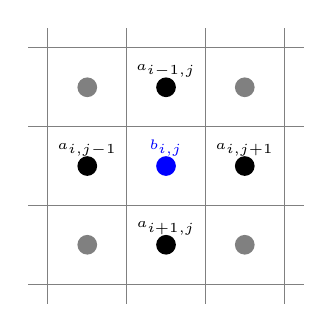
\begin{tikzpicture} [font=\tiny]
		\draw [step=1cm,gray] (-1.25,-1.25) grid (2.25,2.25);
		
		\fill [blue] (.5,.5) circle [radius=.125cm] node [above] {$b_{i,j}$};
		\fill [gray] (-.5,-.5) circle [radius=.125cm];
		\fill [gray] (-.5,1.5) circle [radius=.125cm];
		\fill [gray] (1.5,1.5) circle [radius=.125cm];
		\fill [gray] (1.5,-.5) circle [radius=.125cm];
		\fill [black] (-.5,.5) circle [radius=.125cm] node [above] {$a_{i,j-1}$};
		\fill [black] (.5,1.5) circle [radius=.125cm] node [above] {$a_{i-1,j}$};
		\fill [black] (.5,-.5) circle [radius=.125cm] node [above] {$a_{i+1,j}$};
		\fill [black] (1.5,.5) circle [radius=.125cm] node [above] {$a_{i,j+1}$};
	\end{tikzpicture}
	\end{column}
	
	\begin{column}{8cm}
	Aktualisiere $A$ mit Hilfe von $B$ (Iteration):
	\begin{enumerate}
		\item Simple-IJ
		\begin{lstlisting}
		int i,j;
		
		for(i=1; i<sz-1; i++)
		for(j=1; j<sz-1; j++)
		   b[i][j] = (a[i-1][j] + a[i][j-1] +
		              a[i+1][j] + a[i][j+1])/4.0;

		for(i=1; i<sz-1; i++)
		for(j=1; j<sz-1; j++)
		   a[i][j] = (b[i-1][j] + b[i][j-1] +
		              b[i+1][j] + b[i][j+1])/4.0;
		\end{lstlisting}
	\end{enumerate}
	(Matrizen \texttt{a} und \texttt{b} der Gr"o"se \texttt{sz*sz})
	\end{column}
	
	\end{columns}
\end{frame}

\begin{frame} \frametitle{Jacobi 2} % 1
	\begin{enumerate} \setcounter{enumi}{1}
	\item $A$ und $B$ alternierend zeilenweise durchlaufen (Weave2-IJ)
	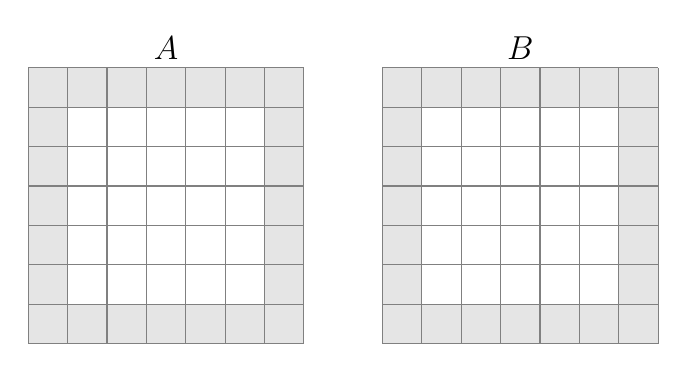
\begin{tikzpicture} [font=\tiny]
		\fill [gray!20] (-1.5,-1.5) rectangle +(.5,3.5);
		\fill [gray!20] (-1.5,-1.5) rectangle +(3.5,.5);
		\fill [gray!20] (-1.5,1.5) rectangle +(3.5,.5);
		\fill [gray!20] (1.5,-1.5) rectangle +(.5,3.5);
		\draw [step=.5cm,gray] (-1.5,-1.5) grid (2,2);
		
		\fill [gray!20] (3,-1.5) rectangle +(.5,3.5);
		\fill [gray!20] (3,-1.5) rectangle +(3.5,.5);
		\fill [gray!20] (3,1.5) rectangle +(3.5,.5);
		\fill [gray!20] (6,-1.5) rectangle +(.5,3.5);
		\draw [step=.5cm,gray] (2.999,-1.5) grid (6.5,2);
		
		\node [font=\large] at (.25,2.25) {$A$};
		\node [font=\large] at (4.75,2.25) {$B$};
	\end{tikzpicture}
	\end{enumerate}
\end{frame}
\begin{frame} \frametitle{Jacobi 2} % 2
	\begin{enumerate} \setcounter{enumi}{1}
	\item $A$ und $B$ alternierend zeilenweise durchlaufen (Weave2-IJ)
	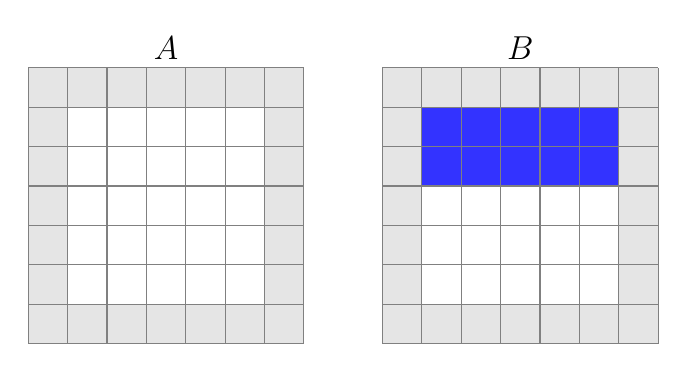
\begin{tikzpicture} [font=\tiny]
		\fill [gray!20] (-1.5,-1.5) rectangle +(.5,3.5);
		\fill [gray!20] (-1.5,-1.5) rectangle +(3.5,.5);
		\fill [gray!20] (-1.5,1.5) rectangle +(3.5,.5);
		\fill [gray!20] (1.5,-1.5) rectangle +(.5,3.5);
		\draw [step=.5cm,gray] (-1.5,-1.5) grid (2,2);
		
		\fill [gray!20] (3,-1.5) rectangle +(.5,3.5);
		\fill [gray!20] (3,-1.5) rectangle +(3.5,.5);
		\fill [gray!20] (3,1.5) rectangle +(3.5,.5);
		\fill [gray!20] (6,-1.5) rectangle +(.5,3.5);
		\fill[blue!80] (3.5,.5) rectangle +(2.5,1);
		\draw [step=.5cm,gray] (2.999,-1.5) grid (6.5,2);
		
		\node [font=\large] at (.25,2.25) {$A$};
		\node [font=\large] at (4.75,2.25) {$B$};
	\end{tikzpicture}
	\end{enumerate}
\end{frame}
\begin{frame} \frametitle{Jacobi 2} % 3
	\begin{enumerate} \setcounter{enumi}{1}
	\item $A$ und $B$ alternierend zeilenweise durchlaufen (Weave2-IJ)
	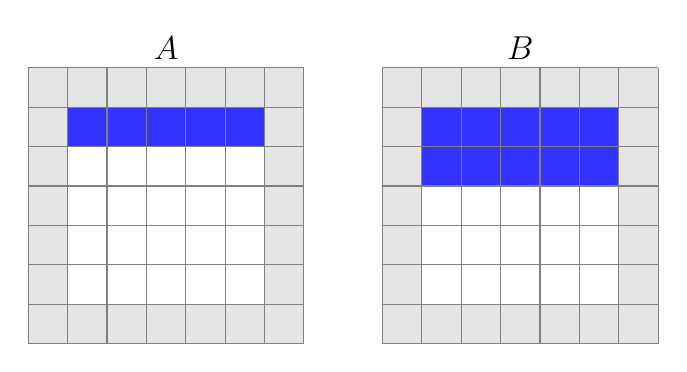
\begin{tikzpicture} [font=\tiny]
		\fill [gray!20] (-1.5,-1.5) rectangle +(.5,3.5);
		\fill [gray!20] (-1.5,-1.5) rectangle +(3.5,.5);
		\fill [gray!20] (-1.5,1.5) rectangle +(3.5,.5);
		\fill [gray!20] (1.5,-1.5) rectangle +(.5,3.5);
		\fill[blue!80] (-1,1) rectangle +(2.5,.5);
		\draw [step=.5cm,gray] (-1.5,-1.5) grid (2,2);
		
		\fill [gray!20] (3,-1.5) rectangle +(.5,3.5);
		\fill [gray!20] (3,-1.5) rectangle +(3.5,.5);
		\fill [gray!20] (3,1.5) rectangle +(3.5,.5);
		\fill [gray!20] (6,-1.5) rectangle +(.5,3.5);
		\fill[blue!80] (3.5,.5) rectangle +(2.5,1);
		\draw [step=.5cm,gray] (2.999,-1.5) grid (6.5,2);
		
		\node [font=\large] at (.25,2.25) {$A$};
		\node [font=\large] at (4.75,2.25) {$B$};
	\end{tikzpicture}
	\end{enumerate}
\end{frame}
\begin{frame} \frametitle{Jacobi 2} % 4
	\begin{enumerate} \setcounter{enumi}{1}
	\item $A$ und $B$ alternierend zeilenweise durchlaufen (Weave2-IJ)
	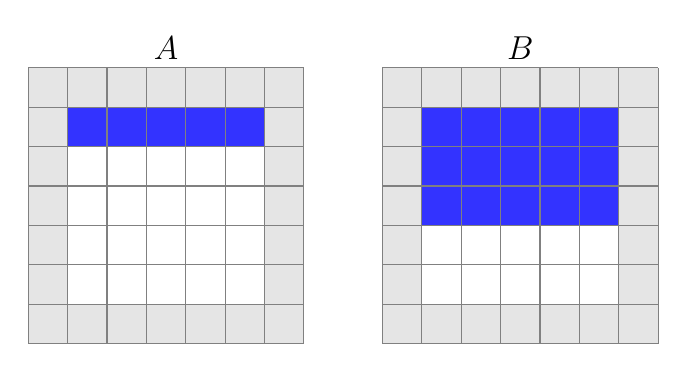
\begin{tikzpicture} [font=\tiny]
		\fill [gray!20] (-1.5,-1.5) rectangle +(.5,3.5);
		\fill [gray!20] (-1.5,-1.5) rectangle +(3.5,.5);
		\fill [gray!20] (-1.5,1.5) rectangle +(3.5,.5);
		\fill [gray!20] (1.5,-1.5) rectangle +(.5,3.5);
		\fill[blue!80] (-1,1) rectangle +(2.5,.5);
		\draw [step=.5cm,gray] (-1.5,-1.5) grid (2,2);
		
		\fill [gray!20] (3,-1.5) rectangle +(.5,3.5);
		\fill [gray!20] (3,-1.5) rectangle +(3.5,.5);
		\fill [gray!20] (3,1.5) rectangle +(3.5,.5);
		\fill [gray!20] (6,-1.5) rectangle +(.5,3.5);
		\fill[blue!80] (3.5,0) rectangle +(2.5,1.5);
		\draw [step=.5cm,gray] (2.999,-1.5) grid (6.5,2);
		
		\node [font=\large] at (.25,2.25) {$A$};
		\node [font=\large] at (4.75,2.25) {$B$};
	\end{tikzpicture}
	\end{enumerate}
\end{frame}
\begin{frame} \frametitle{Jacobi 2} % 5
	\begin{enumerate} \setcounter{enumi}{1}
	\item $A$ und $B$ alternierend zeilenweise durchlaufen (Weave2-IJ)
	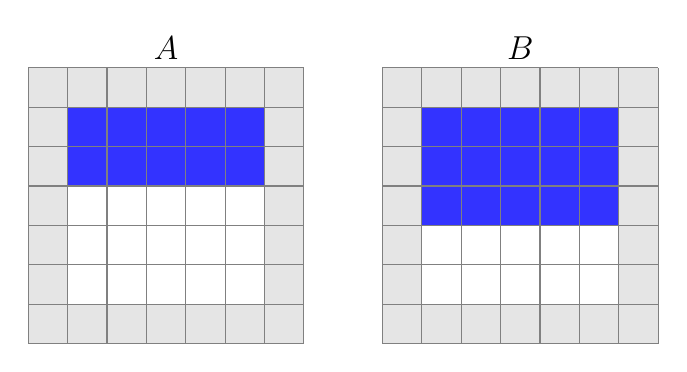
\begin{tikzpicture} [font=\tiny]
		\fill [gray!20] (-1.5,-1.5) rectangle +(.5,3.5);
		\fill [gray!20] (-1.5,-1.5) rectangle +(3.5,.5);
		\fill [gray!20] (-1.5,1.5) rectangle +(3.5,.5);
		\fill [gray!20] (1.5,-1.5) rectangle +(.5,3.5);
		\fill[blue!80] (-1,.5) rectangle +(2.5,1);
		\draw [step=.5cm,gray] (-1.5,-1.5) grid (2,2);
		
		\fill [gray!20] (3,-1.5) rectangle +(.5,3.5);
		\fill [gray!20] (3,-1.5) rectangle +(3.5,.5);
		\fill [gray!20] (3,1.5) rectangle +(3.5,.5);
		\fill [gray!20] (6,-1.5) rectangle +(.5,3.5);
		\fill[blue!80] (3.5,0) rectangle +(2.5,1.5);
		\draw [step=.5cm,gray] (2.999,-1.5) grid (6.5,2);
		
		\node [font=\large] at (.25,2.25) {$A$};
		\node [font=\large] at (4.75,2.25) {$B$};
	\end{tikzpicture}
	usw.
	\end{enumerate}
\end{frame}

